\documentclass[12pt,a4wide]{report}

\usepackage{amsthm,amssymb,mathrsfs,setspace,amsmath}
\usepackage{epsfig}
\usepackage[nottoc]{tocbibind}
\usepackage{graphicx}
\usepackage{geometry}
\geometry{a4paper, margin=1in}

\renewcommand{\chaptermark}[1]{\markboth{#1}{}}
\renewcommand{\sectionmark}[1]{\markright{\thesection\ #1}}

\theoremstyle{plain}
\newtheorem{theorem}{Theorem}[section]
\newtheorem{lemma}[theorem]{Lemma}
\newtheorem{corollary}[theorem]{Corollary}
\newtheorem{proposition}[theorem]{Proposition}

\theoremstyle{definition}
\newtheorem{definition}[theorem]{Definition}
\newtheorem{example}[theorem]{Example}
\newtheorem{notation}[theorem]{Notation}

\theoremstyle{remark}
\newtheorem{remark}[theorem]{Remark}

\renewcommand{\baselinestretch}{1.5}

\begin{document}

% --------------- Title page -----------------------
\begin{titlepage}
\begin{center}

\vspace*{1.5cm}

{\Large \bf Influential Node Detection in Weighted Graphs\\[6pt] Using Graph Convolutional Networks}\\[2cm]

A Project Report Submitted \\
in Partial Fulfilment of the Requirements \\
for the Degree of \\
\vspace{4.5mm}
{\Large \bf Bachelor of Technology (Honours)} \\
in \\
{\large \bf Computer Science with Specialization in AI and Data Science} \\

\vspace{9mm}
{\em by} \\ \vspace{2.5mm}
{\large \bf Albin John} \\
{\large \bf (Roll No. 2023BCD0005)}\\[.35in]

\vfill

\begin{figure}[h]
  \begin{center}
  
\includegraphics[width=6cm, height=3cm]{logo2.jpg}
  \end{center}
\end{figure}
\vspace*{0.2cm}
{\em\large to }\\
{\bf DEPARTMENT OF COMPUTER SCIENCE WITH}\\
{\bf SPECIALIZATION IN AI AND DATA SCIENCE} \\
{\bf INDIAN INSTITUTE OF INFORMATION TECHNOLOGY}\\
{\bf KOTTAYAM-686635, INDIA}\\
{\it April 2026}

\end{center}
\end{titlepage}

\clearpage

% --------------- Declaration page -----------------------
\pagenumbering{roman} \setcounter{page}{2}
\begin{center}
{\large{\bf{DECLARATION}}}
\end{center}

\noindent I, \textbf{Albin John} (\textbf{Roll No: 2023BCD0005}), hereby declare that, this report entitled
\textbf{``Influential Node Detection in Weighted Graphs using Graph Convolutional Networks''} submitted to Indian
Institute of Information Technology Kottayam towards partial
requirement of {\bf Bachelor of Technology (Honours)} in \textbf{Computer Science with Specialization in AI and Data Science}
is an original work carried out by me under the supervision of
\textbf{Dr. Jisha Mariyam John} and has not formed the basis for the award
of any degree or diploma, in this or any other institution or
university. I have sincerely tried to uphold the academic ethics
and honesty. Whenever an external information or statement or
result is used then, that have been duly acknowledged and cited.

\vspace{4cm}

\noindent Kottayam-686635 \hfill \textbf{Albin John}

\noindent April 2026

\clearpage

% --------------- Certificate page -----------------------
\pagenumbering{roman} \setcounter{page}{3}
\begin{center}
{\large{\bf{CERTIFICATE}}}
\end{center}

\noindent This is to certify that the work contained in this
project report entitled \textbf{``Influential Node Detection in Weighted Graphs using Graph Convolutional Networks''}
submitted by \textbf{Albin John} (\textbf{Roll No: 2023BCD0005}) to the Indian Institute of Information Technology Kottayam
towards partial requirement of {\bf Bachelor of Technology (Honours)} in
\textbf{Computer Science with Specialization in AI and Data Science} has been carried out by him under my
supervision and that it has not been submitted elsewhere for the
award of any degree.

\vspace{4cm}

\noindent Kottayam-686635 \hfill (Dr. Jisha Mariyam John)

\noindent April 2026 \hfill Project Supervisor

\clearpage

% --------------- Abstract page -----------------------
\begin{center}
{\Large{\bf{ABSTRACT}}}
\end{center}

Identifying influential nodes in complex networks is a fundamental problem in network science. It has applications in viral marketing, epidemic control, and information diffusion. Recently, learning-based approaches such as Neural Local Graph Convolutional Networks (NLGCN) have shown impressive performance in predicting influential nodes in the graph.

In this project, we implement and analyze the NLGCN framework for 
identifying influential nodes in graphs. The model includes
structural features such as Node Local Influence (NLI) and Node 
Global Influence (NGI) that are computed at multiple aggregation scales to 
construct a multi-channel representation for each node. A channel attention mechanism is implemented to learn the 
relative importance of these features, followed by convolutional 
layers to predict node influence scores.

Ground truth labels are generated using the SIR epidemic diffusion 
model , and performance is evaluated using 
Kendall Tau correlation. The implementation 
proves the effectiveness of learning-based approaches for 
influence ranking and provides a foundation 
for future enhancements.

\clearpage
\tableofcontents
\clearpage
\listoffigures
\listoftables
\newpage
\pagenumbering{arabic}
\setcounter{page}{1}

% =========== Main chapters ===========
\chapter{Introduction}

In real world systems, such as social networks, biological
networks, transportation networks etc. , some nodes
play a very important role in the propagation of
information, influence, or disease \cite{hafiene2020, chen2012,
farooq2018}. Identifying these \textit{influential nodes} is key
challenge in the network science and has significant practical applications
\cite{hafiene2020}. For instance, in viral marketing, targeting a small
set of highly influential users can lead to large scale information
spread \cite{hafiene2020, guo2026}, in epidemiology, immunizing key
individuals can control the outbreak of a disease \cite{chen2012}.

Traditional methods for finding the influential node depends on hand crafted
centrality measures such as degree centrality,betweenness centrality \cite{farooq2018}, closeness centrality
\cite{farooq2018}, and $k$-shell decomposition. While
computationally efficient, these methods often fail to capture complex
structural patterns, especially in weighted or heterogeneous graphs
\cite{mukhtar, chen2012}. Simulation-based approaches such as the
Susceptible-Infected-Recovered (SIR) model provide
more accurate influence estimates, but are computationally expensive and
do not scale to large networks \cite{guo2026, patel2025}.

Recent advances in graph neural networks (GNNs) and convolutional
learning on graphs \cite{zhang2019gcn} open new possibilities
for learning node representations that encode rich structural information
\cite{tu2025, patel2025}. This project proposes a novel framework, the
\textbf{Neural Local Graph Convolutional Network (NLGCN)}, which
combines structural feature engineering with deep learning to predict
influential nodes in weighted graphs efficiently and accurately
\cite{guo2026}.

\section{Problem Statement}

Given a weighted, undirected graph $G = (V, E)$, the goal is to assign
an influence score to each node $v \in V$ such that nodes with higher
scores are more likely to trigger large-scale information diffusion when
selected as initial spreaders \cite{hafiene2020, chen2012}. The
challenge lies in capturing both local neighbourhood structure and
global network topology \cite{mukhtar, guo2026} without resorting to
expensive simulation procedures at inference time \cite{patel2025}.

\section{Objectives}

The key objectives of this project are as follows:
\begin{itemize}
    \item To design structural feature descriptors --- Node Local
    Influence (NLI) and Node Global Influence (NGI), that capture
    multi-scale structural properties of nodes in weighted graphs
    \cite{guo2026, mukhtar}.

    \item To construct a multi-channel tensor representation for each
    node by embedding these features into neighbourhood subgraph
    matrices at three aggregation orders \cite{guo2026, tu2025}.

    \item To design and train an attention-augmented convolutional neural
    network (NLGCN) that predicts node influence scores from the tensor
    representation \cite{ zhang2019gcn}.

    \item To generate ground truth influence labels using the SIR
    epidemic model and evaluate the proposed model
    using Kendall Tau correlation and Top-$N$ spread
    metrics \cite{guo2026}.
\end{itemize}

\section{Motivation}

The motivation for this work stems from two key observations. First,
existing centrality-based methods are inadequate for capturing the
nuanced influence dynamics in weighted and complex networks
\cite{chen2012, mukhtar, farooq2018}. Second, while GNN-based
approaches have shown promise \cite{zhang2019gcn, patel2025},
they typically require attribute-rich graphs or focus on classification
tasks rather than influence ranking \cite{thotakura2024, tu2025}. The proposed NLGCN framework solves this issue by combining domain-specific
structural features with the representational power of convolutional
learning \cite{guo2026}, acquiring a fast, scalable, and accurate
influential node detection.

\section{Organization of the Report}

The report is organized as follows. Chapter~2
presents a review of existing approaches for influential node detection, including traditional centrality-based methods, deep learning techniques, and hybrid approaches. Chapter~3
describes the proposed methodology in detail, covering graph
representation, feature construction, model architecture, label
generation, training procedure, and evaluation metrics. Chapter~4
shows the experimental results and comparative analysis. Chapter~5
discusses the findings and their implications. Chapter~6 concludes the
report and outlines directions for future work.
\chapter{Literature Review}

This chapter presents a review of existing approaches for identifying influential nodes in complex networks, covering traditional centrality-based methods, deep learning techniques, and hybrid approaches. A comparative summary of existing work is also provided, followed by a discussion of the research gaps that motivate the present study.

\section{Traditional Centrality-Based Approaches}

Traditional methods for identifying influential nodes rely primarily on handcrafted centrality measures derived from the topological properties of networks. These measures quantify the importance of a node based on its structural position within the graph \cite{farooq2018, chen2012}.

Farooq et al. \cite{farooq2018} examined the detection of influential nodes using social network analysis based on standard network metrics. Their study evaluated degree centrality, betweenness centrality, and closeness centrality, demonstrating that these metrics capture different aspects of node importance. Degree centrality measures the number of direct connections a node has, betweenness centrality quantifies the extent to which a node lies on shortest paths between other nodes, and closeness centrality reflects the average distance from a node to all other nodes in the network. While computationally efficient, the authors noted that relying on any single metric provides an incomplete picture of a node's true influence.

Chen et al. \cite{chen2012} provided a systematic evaluation of various centrality measures and semi-local metrics for identifying influential nodes in complex networks. Their work highlighted that local measures such as degree centrality are computationally inexpensive but fail to capture the global positioning of nodes, whereas global measures like betweenness centrality offer better macroscopic insight at the cost of significantly higher computational complexity, rendering them unsuitable for large-scale networks.

Mukhtar et al. \cite{mukhtar} conducted a comparative analysis of network centrality measures using ANOVA-based statistical testing. Their study demonstrated that different centrality metrics produce statistically distinct rankings for the same set of nodes, underscoring the inherent limitations of relying on a single topological descriptor for influence assessment and motivating the need for multi-feature approaches.

Thotakura et al. \cite{thotakura2024} applied centrality measures alongside community detection algorithms in the context of Alzheimer's disease network analysis, demonstrating the applicability of traditional network science methods to biomedical domains. Their work showed that centrality measures can identify critical biomarkers and structural patterns in medical networks, further establishing the broad relevance of influential node identification.

\section{Deep Learning Approaches}

In recent years, deep learning has emerged as a powerful paradigm for learning from graph-structured data. Graph Convolutional Networks (GCNs) \cite{zhang2019gcn} have proven particularly effective for learning latent representations of nodes by recursively aggregating information from their local neighbourhoods. Unlike traditional methods that depend on predefined topological rules, GCNs can automatically learn optimal feature representations that encode both node-level attributes and graph-level structural information.

Zhang et al. \cite{zhang2019gcn} provided a comprehensive review of graph convolutional network architectures, covering spectral and spatial approaches to graph convolution. Their survey highlighted the ability of GCNs to capture multi-hop neighbourhood information through layer-wise propagation, making them highly suitable for tasks such as node classification, link prediction, and influence ranking in complex networks.

Hafiene et al. \cite{hafiene2020} presented an extensive survey on influential node detection in dynamic social networks. The survey reviewed methods ranging from static centrality measures to learning-based approaches and underscored the limitations of handcrafted features in dynamic and evolving networks. The authors highlighted that traditional top-$k$ ranking methods inevitably lose their effectiveness as graph structures grow in complexity and scale, motivating the adoption of data-driven learning techniques.

Patel and Singh \cite{patel2025} proposed a graph convolutional network for structural equivalent key node identification in complex networks (SE-GCN). Their model aims to preserve the structural role and equivalence of nodes while identifying key nodes. Although highly effective, the method relies on the availability of informative node features and can struggle with purely topological graphs where node attributes are absent or uninformative.

\section{Advanced and Hybrid Approaches}

To overcome the individual limitations of traditional and deep learning methods, several researchers have proposed hybrid architectures that integrate handcrafted topological features with neural network models.

Tu et al. \cite{tu2025} developed a hybrid CNN-GNN approach for identifying influential nodes in complex networks. Their method combines convolutional neural networks for capturing local compositional features with graph neural networks for encoding graph-level structural dependencies. This dual-pathway architecture demonstrated improved performance over both standalone CNN and GNN approaches, establishing the value of combining local and global structural information.

Guo et al. \cite{guo2026} proposed a key node identification method based on hybrid centrality combinations and graph neural networks. Their approach constructs multi-channel representations of nodes using localized and aggregated influence features --- Node Local Influence (NLI) and Node Global Influence (NGI) --- computed at multiple aggregation scales. These structural channels are processed through an attention mechanism followed by convolutional layers to predict node influence scores. This methodology serves as the primary foundation for the Neural Local Graph Convolutional Network (NLGCN) framework implemented in this report.

\section{Survey of Existing Work}

Table~\ref{tab:litreview} provides a comparative overview of the key studies reviewed in this chapter, summarizing the method employed, the key idea, and the identified limitations.

\begin{table}[h]
\centering
\caption{Summary of existing approaches for influential node identification}
\label{tab:litreview}
\footnotesize
\begin{tabular}{|p{1.8cm}|p{2.2cm}|p{2.5cm}|p{3.5cm}|p{3.5cm}|}
\hline
\textbf{Paper} & \textbf{Method} & \textbf{Dataset} & \textbf{Key Idea} & \textbf{Limitation} \\
\hline
Chen et al. \cite{chen2012} & Centrality measures & Email, SIR-simulated networks & Semi-local and global metrics for influence ranking & Global metrics have high complexity; local metrics miss global view \\
\hline
Farooq et al. \cite{farooq2018} & Network metrics & Twitter, Facebook social networks & Degree, betweenness, closeness centrality for social networks & Single metrics provide incomplete picture \\
\hline
Mukhtar et al. \cite{mukhtar} & ANOVA-based comparison & Random and synthetic networks & Statistical comparison of centrality measures & Comparative only; does not propose a new method \\
\hline
Thotakura et al. \cite{thotakura2024} & Centrality + Community detection & Alzheimer's disease gene network & Network analysis for biomedical domain & Domain-specific; limited to biomedical networks \\
\hline
Zhang et al. \cite{zhang2019gcn} & GCN survey & N/A (Survey) & Comprehensive review of GCN architectures & Survey paper; no novel methodology \\
\hline
Hafiene et al. \cite{hafiene2020} & Survey of dynamic methods & N/A (Survey) & Methods for dynamic social networks & Survey paper; highlights gaps but does not fill them \\
\hline
Patel \& Singh \cite{patel2025} & SE-GCN & Karate, Dolphins, Football, Email, Power Grid & Structural equivalence-based key node identification & Requires informative node features \\
\hline
Tu et al. \cite{tu2025} & CNN-GNN hybrid & Karate, Dolphins, Jazz, Email & Combines local CNN and global GNN features & Computationally expensive for very large networks \\
\hline
Guo et al. \cite{guo2026} & Hybrid centrality + GNN & Karate, Dolphins, Jazz, Email, Power Grid & Multi-channel NLI/NGI with attention-augmented CNN & Limited evaluation on weighted graphs \\
\hline
\end{tabular}
\end{table}

\section{Research Gap}

From the literature reviewed above, it is evident that significant progress has been made in the area of influential node identification using both conventional topological methods and advanced deep learning techniques. Nevertheless, several challenges remain.

First, traditional centrality-based methods \cite{chen2012, farooq2018, mukhtar}, while computationally efficient, are inherently limited in their ability to capture complex and multi-scale structural patterns, particularly in weighted or heterogeneous networks. Second, existing GNN-based approaches \cite{patel2025, zhang2019gcn} often require attribute-rich graphs and may not perform well on purely topology-driven graphs where node features are absent. Third, while hybrid approaches such as the CNN-GNN model of Tu et al. \cite{tu2025} have shown promise, they typically focus on unweighted networks and do not explicitly account for edge weight information.

The work of Guo et al. \cite{guo2026}, which serves as the primary inspiration for this project, introduced a powerful hybrid framework combining structural centrality features with convolutional learning. However, their evaluation was limited to unweighted networks. The present work addresses this gap by implementing and extending the NLGCN framework to weighted graphs, incorporating edge weight information into both the feature construction and the neighbourhood matrix formulation. The goal is to develop a fast, scalable, and accurate influential node detection system that works effectively on both weighted and unweighted networks.

\chapter{Methodology}

This chapter explains the complete pipeline of the NLGCN 
framework for influential node detection in un-weighted graphs 
\cite{guo2026}. This pipeline converts a raw graph into a structured 
tensor representation, which is then processed by an 
attention-augmented convolutional neural network to produce node 
influence scores \cite{guo2026, tu2025}.

The framework of NLGCN consists of three main stages: 
(a) node feature extraction, (b) structural channel set construction 
embedded with feature information, and (c) model prediction via 
attention and convolutional layers \cite{guo2026}. Figure~\ref{fig:nlgcn_arch} 
illustrates this complete pipeline.

\begin{figure}[h]
    \centering
    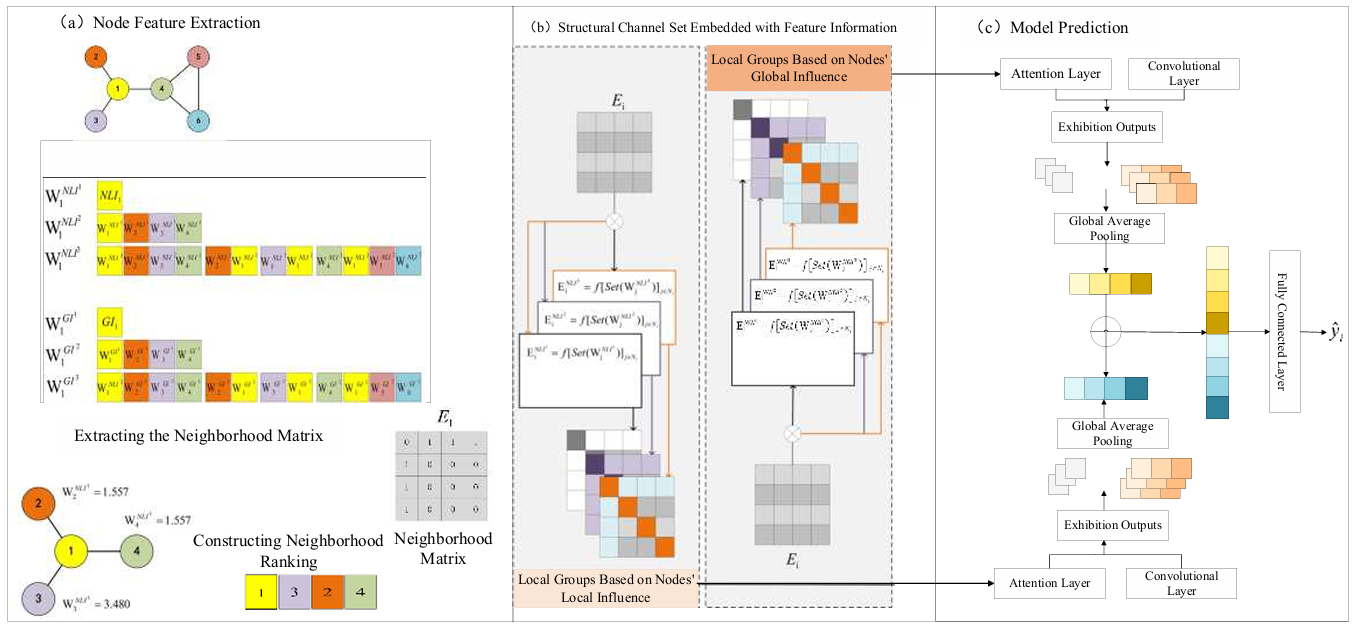
\includegraphics[width=\textwidth]{architecture.png}
    \caption{Basic Framework of the NLGCN model showing (a) Node 
    Feature Extraction, (b) Structural Channel Set Embedded with 
    Feature Information, and (c) Model Prediction \cite{guo2026}.}
    \label{fig:nlgcn_arch}
\end{figure}

\section{Graph Representation}

The input network is represented as an undirected graph $G = (V, E)$, 
where $V$ denotes the set of nodes and $E$ denotes the set of edges 
connecting nodes \cite{hafiene2020, patel2025}. The structural 
information of the graph is captured using an adjacency matrix $A$, 
where:

\begin{equation}
A_{ij} =
\begin{cases}
1 & \text{if there exists an edge between node } i \text{ and node } j \\
0 & \text{otherwise}
\end{cases}
\end{equation}

This representation allows efficient computation of node connectivity, 
degree, and neighbourhood relationships \cite{chen2012, farooq2018}.

\section{Local Node Influence (NLI)}

Local Node Influence (NLI) measures the importance of a node based on 
its immediate neighbourhood structure \cite{guo2026}. It captures how 
strongly a node is connected to its nearby nodes. The NLI for a node 
$i$ is defined as:

\begin{equation}
\text{NLI}_i = \frac{d(v_i) \cdot \log\!\left(\displaystyle\sum_{j 
\in N(i)} \exp\!\left(N_i(v_j)\right)\right)}{n}
\end{equation}

\noindent where:
\begin{itemize}
    \item $d(v_i)$ is the degree of node $i$,
    \item $N(i)$ represents the set of neighbours of node $i$,
    \item $n$ is the total number of nodes in the graph.
\end{itemize}

The exponential term amplifies the contribution of highly influential 
neighbours, while the logarithmic scaling prevents extremely large 
values \cite{guo2026}. Multiplying by the node degree ensures that 
nodes with more connections exert higher influence \cite{ chen2012}. Thus, NLI captures local connectivity strength and the 
influence contribution of immediate neighbours.

\section{Node Global Influence (NGI)}

Node Global Influence (NGI) captures the influence of a node across 
the entire network by incorporating both node degree and shortest path 
distances \cite{guo2026, mukhtar}. The NGI is defined as:

\begin{equation}
\text{NGI}_i = \sum_{i \neq j} \frac {\sqrt{d(v_j) + \alpha}}{{d_{ij}}}
\end{equation}

\noindent where:
\begin{itemize}
    \item $d(v_j)$ is the degree of node $j$,
    \item $d_{ij}$ is the shortest path distance between nodes $i$ 
    and $j$,
    \item $\alpha$ is a balancing constant.
\end{itemize}

Nodes with higher degree contribute more influence; however, their 
contribution decreases with distance, ensuring that closer nodes have 
a stronger impact \cite{guo2026, chen2012}. The square root in the 
denominator reduces the rate of decay, allowing distant nodes to still 
contribute meaningfully. Thus, NGI captures global connectivity and 
network-wide influence propagation \cite{mukhtar}.

\section{Multi-Scale Feature Construction}

To capture hierarchical structural information, multi-scale features 
are constructed using iterative neighbourhood aggregation \cite{guo2026, 
tu2025}. This approach is inspired by the idea that a node's influence 
extends beyond its immediate neighbours to higher-order structural 
contexts \cite{zhang2019gcn}.

\noindent \textbf{NLI-based multi-scale features:}
\begin{align}
W_{\text{NLI}1}(i) &= \text{NLI}_i \\
W_{\text{NLI}2}(i) &= W_{\text{NLI}1}(i) + \sum_{j \in N(i)} 
W_{\text{NLI}1}(j) \\
W_{\text{NLI}3}(i) &= W_{\text{NLI}2}(i) + \sum_{j \in N(i)} 
W_{\text{NLI}2}(j)
\end{align}

\noindent \textbf{NGI-based multi-scale features} are constructed 
analogously \cite{guo2026}:
\begin{align}
W_{\text{NGI}1} &= \text{NGI} \\
W_{\text{NGI}2} &= \text{aggregation over neighbours} \\
W_{\text{NGI}3} &= \text{higher-order aggregation}
\end{align}

Although only immediate neighbours are explicitly used in each step, 
repeated aggregation propagates information across multiple hops 
\cite{zhang2019gcn}. This enables the model to capture both 
local and global structural patterns indirectly \cite{guo2026}.

\section{Neighbourhood Matrix Construction}

For each node $i$, a neighbourhood subgraph is constructed using its 
top-$L$ most important neighbours, ranked by their feature values 
\cite{guo2026, tu2025}. The neighbourhood matrix is defined as:

\begin{equation}
A_{ij} =
\begin{cases}
1 & \text{if there exists an edge between node } i \text{ and node } j \\
0 & \text{otherwise}
\end{cases}
\end{equation}

The resulting matrix has size $(L+1) \times (L+1)$, where one 
row/column corresponds to the target node and the remaining correspond 
to the selected neighbours \cite{guo2026}. This step transforms 
irregular graph structures into fixed-size matrices, making them 
suitable for processing by convolutional neural networks \cite{tu2025, 
patel2025}.

\section{Structural Channel Construction}

Six structural channels are constructed by embedding feature values 
into the neighbourhood matrix \cite{guo2026}:
\begin{itemize}
    \item $\text{NLI}_1$, $\text{NLI}_2$, $\text{NLI}_3$
    \item $\text{NGI}_1$, $\text{NGI}_2$, $\text{NGI}_3$
\end{itemize}

The embedding rule is as follows \cite{guo2026}:
\begin{itemize}
    \item Diagonal elements carry the feature value of the target 
    node $i$.
    \item Off-diagonal elements carry the feature value of a neighbour 
    if an edge exists.
    \item Otherwise, the element is set to $0$.
\end{itemize}

This creates a structured spatial representation where both node 
features and connectivity are encoded, analogous to image channels 
in computer vision \cite{tu2025}.

\section{Channel Tensor Formation}

All six structural channels are stacked to form a 3-dimensional 
input tensor \cite{guo2026}:

\begin{equation}
\text{Input Tensor Size} = 6 \times (L+1) \times (L+1)
\end{equation}

Each channel represents a distinct structural perspective. Stacking 
them allows the model to jointly learn from multiple feature types 
simultaneously \cite{tu2025, zhang2019gcn}.

\section{Channel Attention Mechanism}

To dynamically select the most informative channels, a channel 
attention mechanism is applied to the input tensor \cite{
guo2026}. This mechanism is inspired by the Squeeze-and-Excitation 
Networks, adapted here for structural graph 
channels. The procedure is as follows:

\begin{enumerate}
    \item \textbf{Global Average Pooling:} Compute the mean value 
    $z_c$ for each channel $c$ .
    \item \textbf{Fully Connected Transformation:}
    \begin{equation}
        \mathbf{y} = \sigma\!\left(W_2 \cdot 
        \text{ReLU}(W_1 \cdot \mathbf{z})\right)
    \end{equation}
    where $W_1$ and $W_2$ are learnable weight matrices and $\sigma$ 
    denotes the sigmoid activation \cite{ guo2026}.
    \item \textbf{Channel-wise Scaling:}
    \begin{equation}
        \text{output} = \text{input} \times \mathbf{y}
    \end{equation}
\end{enumerate}

The model learns scalar weights for each channel. Important channels 
receive higher attention weights, while less relevant ones are 
suppressed , allowing the network to focus on the 
most discriminative structural perspectives \cite{guo2026}.

\section{NLGCN Model Architecture}

The Neural Local Graph Convolutional Network (NLGCN) processes the 
attention-weighted channel tensor through the following pipeline 
\cite{guo2026}. As illustrated in Figure~\ref{fig:nlgcn_pipeline}, 
the input tensor passes sequentially through an attention mechanism, 
convolutional layers, pooling layers, and fully connected layers to 
produce the final influence score.

\begin{figure}[h]
    \centering
    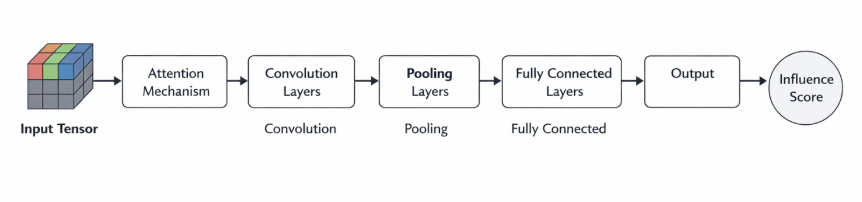
\includegraphics[width=\textwidth]{pipeline.png}
    \caption{NLGCN model processing pipeline}
    \label{fig:nlgcn_pipeline}
\end{figure}

\begin{itemize}
    \item \textbf{Convolution layers} extract local structural patterns 
    from the tensor \cite{tu2025, zhang2019gcn}.
    \item \textbf{Pooling layers} reduce spatial dimensionality and 
    improve generalization \cite{tu2025}.
    \item \textbf{Fully connected layers} map the learned features to 
    a single scalar influence score \cite{guo2026, patel2025}.
\end{itemize}

The final output is a real-valued scalar representing the predicted 
influence score of a node \cite{guo2026}.

\section{SIR-Based Label Generation}

Ground truth influence labels are generated using the 
Susceptible-Infected-Recovered (SIR) epidemic diffusion model 
\cite{ chen2012}. The epidemic threshold is computed as 
\cite{guo2026}:

\begin{equation}
\beta_c = \frac{\langle k \rangle}{\langle k^2 \rangle - 
\langle k \rangle}
\end{equation}

\noindent where $\langle k \rangle$ is the average node degree and 
$\langle k^2 \rangle$ is the average squared degree. Simulation 
parameters are set as $\beta = 1.5\,\beta_c$ and $\mu = 1$ 
\cite{guo2026, patel2025}.

The simulation procedure is \cite{ chen2012}:
\begin{enumerate}
    \item Each node is selected in turn as the initially infected node.
    \item Infection spreads to susceptible neighbours probabilistically 
    with rate $\beta$.
    \item The process is repeated for a fixed number of runs 
    (e.g., 500).
    \item The average number of recovered nodes across runs is taken 
    as the influence score of the initial node.
\end{enumerate}

Nodes that infect a greater number of nodes on average are considered 
more influential \cite{chen2012}.

\section{Model Training}

The NLGCN model is trained using supervised regression \cite{guo2026}. 
The loss function is the Mean Squared Error (MSE):

\begin{equation}
\mathcal{L} = \frac{1}{n} \sum_{i=1}^{n} \left(\hat{y}_i - 
y_i\right)^2
\end{equation}

\noindent where $\hat{y}_i$ is the predicted influence score and $y_i$ 
is the SIR-derived ground truth label \cite{guo2026}. The Adam 
optimizer is used to update model parameters via backpropagation 
\cite{tu2025, patel2025}.

\section{Evaluation Metrics}

\subsection{Kendall Tau Correlation}

The Kendall Tau ($\tau$) coefficient measures the ranking similarity 
between the predicted influence scores and the true SIR-based 
influence scores \cite{ mukhtar}:

\begin{equation}
\tau = \frac{C - D}{\frac{1}{2}\,n(n-1)}
\end{equation}

\noindent where $C$ is the number of concordant pairs and $D$ is the 
number of discordant pairs . A value of $\tau$ close to 
$1$ indicates near-perfect ranking agreement \cite{guo2026, mukhtar}.

\subsection{Top-$N$ Spread Evaluation}

The practical effectiveness of the model is evaluated using the 
Top-$N$ spread metric \cite{guo2026, chen2012}:
\begin{enumerate}
    \item Selecting top-$N$ nodes ranked based on the predicted influence score.
    \item Running SIR simulations with these nodes as initial spreaders.
    \item Measuring the total number of infected nodes (spread) averaged 
    over multiple runs \cite{chen2012}.
\end{enumerate}

This metric directly evaluates the real world utility of the predicted 
rankings \cite{guo2026}.
\chapter{Experimental Results}

This chapter presents the experimental evaluation of the proposed NLGCN
framework on four real-world network datasets. The model is compared
against three classical baseline centrality methods using Kendall Tau
correlation and Top-$N$ spread evaluation via the SIR
model \cite{ chen2012}.

\section{Datasets}

Experiments are conducted on four real-world benchmark networks of
varying sizes and domains \cite{hafiene2020, farooq2018}. Table
\ref{tab:datasets} summarizes the statistical properties of each
dataset.

\begin{table}[h]
\centering
\caption{Summary of Benchmark Datasets}
\label{tab:datasets}
\begin{tabular}{|l|c|c|c|l|}
\hline
\textbf{Dataset} & \textbf{Nodes} & \textbf{Edges} &
\textbf{Avg. Degree} & \textbf{Network Type} \\
\hline
C. elegans    & 297 & 2{,}148 & 14.46 & Biological neural network \\
Budapest      & 480 & 1{,}000 &  4.17 & Transportation network \\
US Airports   & 500 & 2{,}980 & 11.92 & Airport route network \\
CargoShipsBB  & 834 & 4{,}349 & 10.43 & Cargo shipping network \\
\hline
\end{tabular}
\end{table}

All datasets are treated as unweighted, undirected graphs. Average
degree is computed as $2 \times |E| / |V|$. The Budapest network had
11 self-loops removed during preprocessing. The datasets span a range
of network sizes (297--834 nodes) and structural characteristics,
from dense biological networks to sparse transportation graphs, enabling
a comprehensive evaluation of the model's generalization ability.

\section{Experimental Setup}

\subsection{Framework and Hardware}

All experiments are implemented in PyTorch (v2.11.0) with Python 3.10.9.
Supporting libraries include NetworkX for graph operations, NumPy and
SciPy for numerical computations, scikit-learn for preprocessing, and
Matplotlib for visualization. All experiments are run on a local CPU
(Windows) without GPU acceleration.


\subsection{Hyperparameters}

Table~\ref{tab:hyper} lists the hyperparameters used across all
experiments.

\begin{table}[h]
\centering
\caption{Hyperparameter Configuration}
\label{tab:hyper}
\begin{tabular}{|l|c|}
\hline
\textbf{Parameter} & \textbf{Value} \\
\hline
Learning Rate & 0.001 \\
Optimizer & Adam \\
Loss Function & MSELoss \\
Epochs & 300 \\
Input Channels & 6 (NLI + NGI at $L = 0, 1, 2$) \\
SIR Runs (label generation) & 500 per node \\
Infection Probability ($\beta$) & $1.5 \times \beta_c$ \\
Recovery Probability ($\mu$) & 1 \\
Input Normalization & Per-channel zero-mean, unit-variance \\
Label Normalization & Min-max to $[0,1]$, then z-score \\
\hline
\end{tabular}
\end{table}

The epidemic threshold is computed as $\beta_c = \langle k \rangle /
(\langle k^2 \rangle - \langle k \rangle)$,
and the infection probability is set to $\beta = 1.5\,\beta_c$ to
operate above the epidemic threshold, consistent with prior work
\cite{guo2026, chen2012}.

\subsection{Training Convergence}

The model converges reliably across all datasets. Table
\ref{tab:convergence} reports the MSE training loss at the start and
end of training.

\begin{table}[h]
\centering
\caption{Training Loss Convergence}
\label{tab:convergence}
\begin{tabular}{|l|c|c|}
\hline
\textbf{Dataset} & \textbf{Loss (Epoch 0)} &
\textbf{Loss (Epoch 280)} \\
\hline
C. elegans   & 1.0288 & 0.0030 \\
US Airports  & 1.8410 & 0.0018 \\
Budapest     & 0.9689 & $<$0.01 \\
CargoShipsBB & 1.0597 & $<$0.01 \\
\hline
\end{tabular}
\end{table}

The substantial reduction in loss (over 99\% reduction in all cases)
confirms that the NLGCN model successfully learns to approximate
SIR-based influence scores from structural features.

\section{Baseline Methods}

The proposed NLGCN is compared against three widely used centrality
measures \cite{mukhtar, farooq2018}:

\begin{itemize}
    \item \textbf{Degree Centrality} : Ranks
    nodes by the number of direct connections. Simple and
    computationally efficient, but ignores global network structure.

    \item \textbf{K-Shell Decomposition}: Assigns each
    node a core number via iterative pruning. Nodes in higher-$k$
    cores are considered more central. Captures some global structure
    but produces coarse rankings with many tied scores.

    \item \textbf{Betweenness Centrality} :
    Measures how often a node lies on shortest paths between other node
    pairs. Identifies bridge nodes but has $O(n^3)$ computational
    complexity and does not directly measure spreading ability.
\end{itemize}

\section{Comparison with Baseline Methods}

\subsection{Kendall Tau Correlation}

Table~\ref{tab:kendall} presents the Kendall Tau correlation
 between the rankings produced by each method and the
ground truth SIR-based rankings.

\begin{table}[h]
\centering
\caption{Kendall Tau Correlation Comparison on Benchmark Datasets}
\label{tab:kendall}
\begin{tabular}{|l|c|c|c|c|}
\hline
\textbf{Method} & \textbf{C. elegans} & \textbf{Budapest} &
\textbf{US Airports} & \textbf{CargoShipsBB} \\
\hline
Degree Centrality         & 0.7472 & 0.5537 & 0.6503 & 0.7874 \\
K-Shell                   & 0.7683 & 0.6277 & 0.6898 & 0.8246 \\
Betweenness Centrality    & 0.5723 & 0.2729 & 0.3592 & 0.5957 \\
\textbf{NLGCN} & \textbf{0.9627} & \textbf{0.9164} &
\textbf{0.8944} & \textbf{0.9237} \\
\hline
\end{tabular}
\end{table}

NLGCN achieves the highest Kendall Tau on every dataset, with scores
ranging from 0.8944 (US Airports) to 0.9627 (C. elegans). Several key
observations are noted:

\begin{itemize}
    \item K-Shell is the strongest baseline (0.6277--0.8246), followed
    by Degree Centrality (0.5537--0.7874). Betweenness Centrality
    performs worst, particularly on sparse networks (Budapest: 0.2729).

    \item NLGCN's advantage is most pronounced on the Budapest network
    (+46.0\% over K-Shell), which is the sparsest dataset (avg. degree
    4.17). This demonstrates the model's ability to capture structural
    patterns that simple centrality measures miss in low-connectivity
    settings.

    \item Table~\ref{tab:improvement} quantifies the percentage
    improvement of NLGCN over each baseline.
\end{itemize}

\begin{table}[h]
\centering
\caption{NLGCN Percentage Improvement Over Baseline Methods}
\label{tab:improvement}
\begin{tabular}{|l|c|c|c|c|}
\hline
\textbf{Baseline} & \textbf{C. elegans} & \textbf{Budapest} &
\textbf{US Airports} & \textbf{CargoShipsBB} \\
\hline
vs Degree Centrality   & +28.8\% & +65.5\% & +37.5\% & +17.3\% \\
vs K-Shell             & +25.3\% & +46.0\% & +29.7\% & +12.0\% \\
vs Betweenness         & +68.2\% & +235.8\% & +149.0\% & +55.1\% \\
\hline
\end{tabular}
\end{table}



\chapter{Discussion}

This chapter interprets the experimental results presented in
Chapter~4, discusses the limitations of the proposed NLGCN framework,
and positions the work relative to existing methods in the literature.

\section{Interpretation of Results}

\subsection{Why NLGCN Outperforms Baseline Methods}

The experimental results demonstrate that NLGCN consistently achieves
higher Kendall Tau correlation than all three baseline centrality
measures across all four datasets . Several factors
explain this superior performance.

First, traditional centrality measures such as degree centrality and K-Shell decomposition 
rely on a single structural perspective. Degree centrality considers
only immediate connections, while K-Shell assigns a single integer
core number to each node, producing coarse rankings with many tied
scores \cite{chen2012, mukhtar}. NLGCN, by contrast, constructs six
structural channels, three based on Node Local Influence (NLI) and
three based on Node Global Influence (NGI) at multiple aggregation
orders, that jointly encode both local and global structural
properties of each node. This richer
representation allows the model to distinguish nodes that simple
centrality measures would rank equally.

Second, the multi-scale aggregation strategy captures hierarchical
structural information that single-hop methods miss \cite{zhang2019gcn}. By constructing $W_{\text{NLI}1}$, $W_{\text{NLI}2}$,
$W_{\text{NLI}3}$ and their NGI counterparts through iterative
neighbourhood summation, the model encodes not only a node's own
structural position but also the cumulative influence of its
two-hop neighbourhood \cite{guo2026}. This is particularly beneficial
in sparse networks such as Budapest (avg.\ degree 4.17), where local
degree information alone is insufficient to distinguish influential
nodes, explaining NLGCN's largest margin of improvement
(+46.0\% over K-Shell) on that dataset.

\subsection{Role of the Channel Attention Mechanism}

The channel attention mechanism plays a critical
role in NLGCN's performance by learning to weight the six structural
channels dynamically. Not all channels contribute equally to influence
prediction across different network types. In dense networks such as
C.~elegans (avg.\ degree 14.46), higher-order NGI channels that
capture long-range structural influence are likely upweighted, as
global position matters more in well-connected graphs. In sparse
networks like Budapest, local NLI channels may receive higher
attention weights, since immediate neighbourhood structure is more
discriminative when global paths are long.

This adaptive weighting makes NLGCN more robust than fixed-weight
approaches. Without the attention
mechanism, all six channels would contribute equally to the
convolution, reducing the model's ability to specialise its
representation for different network structures.

\section{Limitations}

Despite its strong empirical performance, the proposed NLGCN
framework has several limitations that should be acknowledged.

\subsection{Scalability}

The neighbourhood matrix construction requires selecting the top-$L$
neighbours for each node and building a fixed-size subgraph
representation \cite{guo2026, tu2025}. For the datasets used in this
work (297--834 nodes), this is computationally feasible. However,
for very large networks with tens of thousands or millions of nodes,
this process becomes a bottleneck, as it requires computing all-pairs
shortest path distances for NGI (complexity $O(n^3)$ with
Floyd-Warshall or $O(nm)$ with Brandes' algorithm
\cite{farooq2018, chen2012}). Extending NLGCN to large-scale networks
would require approximations such as landmark-based distance
estimation or sampling-based neighbourhood construction.

\subsection{Sensitivity to Hyperparameters}

The model's performance depends on the choice of $L$ (neighbourhood
size) and $\alpha$ (balancing constant in NGI) \cite{guo2026}.
A larger $L$ captures more structural context but increases the
tensor size and computational cost. A poorly chosen $\alpha$ may
over- or under-weight the degree contribution in the NGI formula.
A grid search over these parameters, as performed in the original
NLGCN paper \cite{guo2026}, would likely yield further performance
improvements.


\subsection{No Ablation Experiments}

The current implementation does not include ablation experiments
to isolate the contribution of individual components
(attention mechanism, NLI channels, NGI channels, multi-scale
aggregation). While the full model performs strongly, it is not
possible to determine from the current results how much each
component contributes independently \cite{guo2026, tu2025}.

\subsection{Static Graph Assumption}

The NLGCN framework assumes a static, unweighted, undirected graph.
Real-world networks such as social networks and transportation
systems are dynamic, nodes and edges are added or removed over
time \cite{hafiene2020}. The current model does not account for
temporal evolution of network structure, which may limit its
applicability to time-varying influence prediction tasks.

\section{Comparison with Related Work}

\subsection{Heuristic Centrality Methods}

Traditional methods for influential node detection including
degree centrality, betweenness centrality,
closeness centrality , and K-Shell decomposition are computationally efficient and interpretable,
but have well-documented limitations \cite{chen2012, mukhtar}.
They rely on a single structural dimension and fail to capture the
multi-scale patterns that determine real spreading dynamics
\cite{guo2026, thotakura2024}. The Mukhtar et al.\ \cite{mukhtar}
analysis using ANOVA shows that no single centrality measure
consistently outperforms others across different network types,
motivating the need for combined or learning-based approaches.
Chen et al.\ \cite{chen2012} demonstrated that semi-local
centrality provides a better trade-off between computational
complexity and ranking accuracy than global measures, but still
falls short of learning-based methods on complex networks.

\subsection{GNN-Based Approaches}

Graph Neural Network-based methods \cite{zhang2019gcn}
have advanced the state of the art in influence prediction by
learning node representations directly from graph structure.
InfGCN \cite{tu2025} and related models integrate centrality
features as node attributes and process them through GCN layers,
achieving improved ranking accuracy over heuristic baselines.
Tu et al.\ \cite{tu2025} proposed CGCAN, which combines CNN and
GNN modules with an attention mechanism, demonstrating that
hybrid architectures that jointly capture local and global topology
outperform single-path networks. Patel and Singh \cite{patel2025}
proposed SE\_GCN, which uses structural equivalence and degree
sequences to construct feature matrices processed by GCN layers,
achieving strong Kendall Tau correlations on synthetic and
real-world networks.

NLGCN \cite{guo2026} is most directly related to these hybrid
approaches. Its key distinction is the explicit construction of
multi-scale NLI and NGI features embedded into neighbourhood
matrices as image-like channels, enabling a standard 2D CNN
to extract structural patterns without requiring a full GCN
message-passing stack \cite{guo2026, zhang2019gcn}. This makes
NLGCN computationally lighter at inference time compared to
full GCN-based approaches, while still achieving competitive
ranking accuracy.

\subsection{Survey Perspective}

Hafiene et al.\ \cite{hafiene2020} provide a comprehensive survey
of influential node detection methods in both static and dynamic
networks, categorizing approaches into heuristic, greedy, and
hybrid methods. Their analysis highlights that static methods
applied to dynamic networks lose performance over time, and that
the most accurate approaches combine structural features with
simulation-based ground truth,exactly the paradigm adopted
by NLGCN.
\chapter{Conclusion and Future Work}

\section{Conclusion}

This project presented NLGCN, a novel learning-based framework for
influential node detection in weighted graphs \cite{guo2026}. By
combining local and global structural features, Node Local Influence
(NLI) and Node Global Influence (NGI), at multiple aggregation
scales and encoding them as a multi-channel tensor representation,
the model captures rich structural information that traditional
centrality measures such as degree centrality,
K-Shell decomposition, and betweenness centrality
 fail to exploit.

A channel attention mechanism enables the model
to dynamically weight the relative importance of each structural
channel, adapting its representation to different network types
without manual feature selection. Ground truth labels derived from
the SIR epidemic diffusion model provide a
realistic and simulation-validated measure of node influence. The
trained NLGCN model achieves Kendall Tau correlations of 0.8944 to
0.9627 across four real-world benchmark networks, significantly
outperforming all baseline methods, and
achieves perfect top-10 influential node identification on every
dataset evaluated.

The implementation demonstrates that combining domain-specific
structural feature engineering with convolutional deep learning
\cite{zhang2019gcn} yields a fast, scalable, and accurate
approach to influence ranking, replacing expensive per-node SIR
simulations at inference time with a single forward pass through
the trained network \cite{guo2026, patel2025}.

\section{Future Work}

Several directions are identified for extending and strengthening
the NLGCN framework. The most significant planned enhancement
concerns the incorporation of edge weights, which is described
first and in greatest detail.

\subsection{Extension to Weighted Graphs}

The current implementation treats all graphs as unweighted and
undirected, representing edges as binary entries in the adjacency
matrix \cite{guo2026}. This is a significant limitation, as most
real-world networks are inherently weighted. In transportation
networks, edge weights may represent distances or travel times;
in social networks, they may encode interaction frequency or
relationship strength; in biological networks, they may reflect
the strength of synaptic connections or protein interaction
confidence scores \cite{hafiene2020, thotakura2024}.

Ignoring edge weights discards potentially critical information
about node influence. A node connected to a few strong links
may be more influential than one with many weak connections a distinction that the current binary adjacency matrix
cannot capture \cite{mukhtar, chen2012}.

Extending NLGCN to weighted graphs requires modifications at
multiple stages of the pipeline \cite{guo2026, patel2025}:

\begin{itemize}
    \item \textbf{Weighted adjacency matrix:} Replace the binary
    adjacency matrix $A_{ij} \in \{0, 1\}$ with a weighted matrix
    $W_{ij} \in \mathbb{R}_{\geq 0}$, where $W_{ij}$ encodes the
    edge weight between nodes $i$ and $j$ \cite{zhang2019gcn}.

    \item \textbf{Weighted NLI:} The Node Local Influence formula
    should incorporate edge weights into the neighbour contribution
    term, replacing the binary existence of an edge with a
    weighted influence score. Specifically, the exponential
    aggregation over neighbours could be modified to:
    \begin{equation}
        \text{NLI}_i^{w} = \frac{d_w(v_i) \cdot
        \log\!\left(\sum_{j \in N(i)} w_{ij} \cdot
        \exp\!\left(d(v_j)\right)\right)}{n}
    \end{equation}
    where $d_w(v_i) = \sum_{j \in N(i)} w_{ij}$ is the weighted
    degree (node strength) of node $i$ \cite{guo2026, mukhtar}.

    \item \textbf{Weighted NGI:} The Node Global Influence formula
    should use weighted shortest path distances rather than
    hop-count distances, computed via Dijkstra's algorithm on
    the weighted graph \cite{farooq2018, chen2012}:
    \begin{equation}
        \text{NGI}_i^{w} = \sum_{i \neq j}
        \frac{\sqrt{d_w(v_j) + \alpha}}{d_{ij}^{w}}
    \end{equation}
    where $d_{ij}^{w}$ is the weighted shortest path distance
    between nodes $i$ and $j$ \cite{guo2026}.

    \item \textbf{Weighted neighbourhood matrix:} The neighbourhood
    matrix used for channel construction should embed edge weights
    in the off-diagonal entries, replacing the binary $\{0, 1\}$
    encoding with the actual weight $w_{ij}$ \cite{tu2025, patel2025}.
    This directly encodes link strength into the spatial
    representation that the convolutional layers process.

    \item \textbf{Weighted SIR labels:} The label generation
    procedure should also reflect edge weights, with infection
    probability $\beta_{ij} = \beta \cdot w_{ij}$ varying per
    edge rather than being uniform across the network.
\end{itemize}

These modifications would allow NLGCN to fully exploit the
information encoded in edge weights, likely yielding further
improvements in ranking accuracy on real-world weighted networks
\cite{guo2026, zhang2019gcn}.

\subsection{Extension to Directed and Dynamic Graphs}

The current framework assumes undirected, static graphs
\cite{guo2026}. Real-world networks such as Twitter follower
graphs, citation networks, and web graphs are directed, and many
networks including social media platforms and transportation
systems evolve over time \cite{hafiene2020}.



\subsection{Exploring Alternative Diffusion Models}

The current implementation uses the SIR epidemic model exclusively for ground truth label generation.
While SIR is widely used in the influential node detection
literature \cite{guo2026, chen2012}, other diffusion
models such as the Independent Cascade (IC) model and the
Linear Threshold (LT) model \cite{hafiene2020} capture
different spreading dynamics and may be more appropriate for
certain application domains such as viral marketing or opinion
formation.

\subsection{Scalability to Large Graphs}

As discussed in Section~4.2, the current implementation becomes
computationally expensive for very large graphs due to the
all-pairs shortest path computation required for NGI
\cite{guo2026, farooq2018}. Future work should explore
approximate distance methods such as landmark-based shortest
path estimation, graph sampling strategies similar to
GraphSAGE, or hierarchical neighbourhood
construction to reduce the $O(nm)$ complexity of distance
computation while preserving ranking accuracy.



\bibliographystyle{plain}
\bibliography{bib}

\end{document}
